Geometrically, in the x-y plane, \textbf{T} is the reflection about the diagonal x = y and \textbf{U} is a projection onto the x-axis.\\ 
\begin{enumerate}
	\item Reflection
%\end{enumerate}
\begin{align}
\intertext{Let Consider Matrix A as} \vec{A} = \myvec{0 & 1 \\ 1 & 0 } 
\end{align}
The matrix  $\vec{A}$ is representation  of the linear transformation T across the line y=x with respect to the standard basis.
\begin{align}
\intertext{Let suppose}\vec{x_1} =\myvec{x_1 \\ x_2} = \myvec{1 \\ 2},\vec{x_2} =\myvec{x_1 \\ x_2} =\myvec{3 \\ 4} 
\end{align}
After applying linear operator \textbf{T} on it,

\begin{align}
\textbf{T}\brak{x_1, x_2} = \vec{A}\myvec{ x_1  \\ x_2}\\
\implies   \vec{A}\myvec{1 \\ 2} =  \myvec{0 & 1 \\ 1 & 0 } \myvec{1 \\ 2} = \myvec{2 \\ 1}\\
\intertext{Similarly}
  \vec{A}\myvec{3 \\ 4} =  \myvec{0 & 1 \\ 1 & 0 } \myvec{3 \\ 4} = \myvec{4 \\ 3}
  \end{align}
  Hence after  applying Operator \textbf{T} on $\vec{x_1}$ and $\vec{x_2}$
  \begin{align}
  \vec{x_1} = \myvec{2\\1}, \vec{x_2} =\myvec{4\\3}
\end{align}
\begin{figure}[htb!]	
	\centering	
	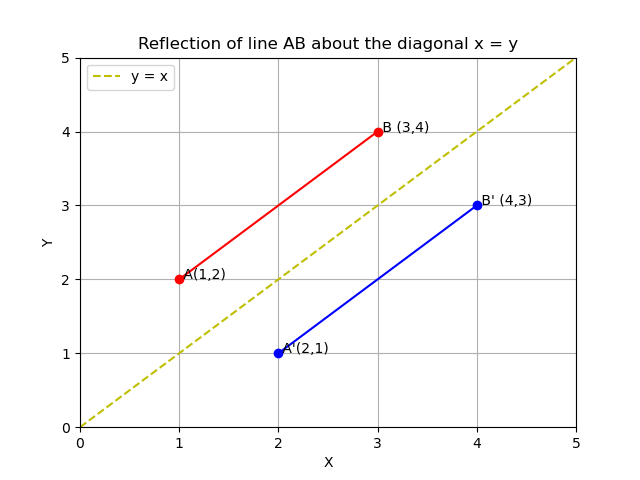
\includegraphics[width=\columnwidth]{./solutions/3/2/1/a/Python_Code/Reflection.png}	
	\caption{Reflection of line AB about the  x = y}
	\label{eq:solutions/3/2/1/a/fig1}	
\end{figure}
%\begin{enumerate}
\item Projection
\end{enumerate}
\begin{align}
\intertext{ For projection let Consider Matrix B as} \vec{B} = \myvec{1 & 0 \\ 0 & 0 } 
\end{align}
The matrix  $\vec{B}$ is representation  of the linear transformation \textbf{U} that is projection on x-axis.
\begin{align}
\intertext{Let suppose}\vec{x_1} =\myvec{x_1 \\ x_2} = \myvec{1 \\ 2},\vec{x_2} =\myvec{x_1 \\ x_2} =\myvec{3 \\ 4} 
\end{align}
After applying linear operator \textbf{U} on $\vec{x_1}$ and $x_2$,

\begin{align}
\textbf{T}\brak{x_1, x_2} = \vec{U}\myvec{ x_1  \\ x_2}\\
\implies   \vec{B}\myvec{1 \\ 2} =  \myvec{1 & 0 \\ 0 & 0 } \myvec{1 \\ 2} = \myvec{1 \\ 0}\\
\intertext{Similarly}
\vec{A}\myvec{3 \\ 4} =  \myvec{1 & 0 \\ 0 & 0 } \myvec{3 \\ 4} = \myvec{3 \\ 0}
\end{align}

\begin{figure}[htb!]	
	\centering	
	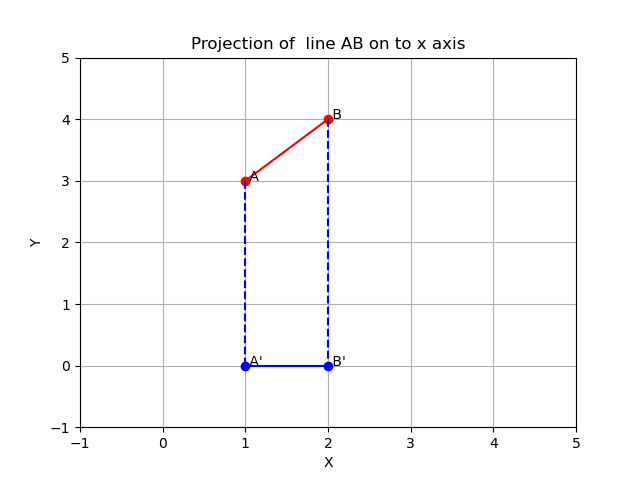
\includegraphics[width=\columnwidth]{./solutions/3/2/1/a/Python_Code/projection.png}	
	\caption{Projection of AB onto x-axis}
	\label{eq:solutions/3/2/1/a/fig2}	
\end{figure}
Hence after  applying Operator \textbf{U} on $\vec{x_1}$ and $\vec{x_2}$
\begin{align}
\vec{x_1} = \myvec{1\\0}, \vec{x_2} =\myvec{3\\0}
\end{align}




